%
%  THESISBOEK
%
%  Dit bestand zorgt voor algemene (layout)definities, en groepeert de
%  afzonderlijke LaTeX-files tot een geheel.
%
%  @author Erwin Six, David De Reu, Brecht Vermeulen
%

\documentclass[11pt,a4paper,oneside,notitlepage]{book}
\usepackage[english]{babel}
\usepackage{algorithmic}
\usepackage{algorithm}
\usepackage{amsthm}
\usepackage{hyperref}
\usepackage{array}
%\usepackage[nottoc]{tocbibind} % Bibliografie in ToC; zie tocbibind.dvi

% marges aanpassen
% (opmerking: moet *voor* inclusie van fancyhdr package komen)
\setlength{\hoffset}{-1in}
\setlength{\voffset}{-1in}
\setlength{\topmargin}{2cm}
\setlength{\headheight}{0.5cm}
\setlength{\headsep}{1cm}
\setlength{\oddsidemargin}{3.5cm}
\setlength{\evensidemargin}{3.5cm}
\setlength{\textwidth}{16cm}
\setlength{\textheight}{23.3cm}
\setlength{\footskip}{1.5cm}

\usepackage{fancyhdr}
\usepackage{graphicx}
% \usepackage[colorlinks]{hyperref}
% Het bibliografisch opmaak bestand.
\bibliographystyle{unsrt}
%\bibliographystyle{bibliodutch}
%\bibpunct{[}{]}{,}{n}{,}{,}

\newtheorem{mydef}{Definition}
\newtheorem{foundation}{Foundation}

\pagestyle{fancy}

\renewcommand{\chaptermark}[1]{\markright{\MakeUppercase{#1}}}
\renewcommand{\sectionmark}[1]{\markright{\thesection~#1}}

\newcommand{\headerfmt}[1]{\textsl{\textsf{#1}}}
\newcommand{\headerfmtpage}[1]{\textsf{#1}}

\fancyhf{}
\fancyhead[LE,RO]{\headerfmtpage{\thepage}}
\fancyhead[LO]{\headerfmt{\rightmark}}
\fancyhead[RE]{\headerfmt{\leftmark}}
\renewcommand{\headrulewidth}{0.5pt}
\renewcommand{\footrulewidth}{0pt}

\fancypagestyle{plain}{ % eerste bladzijde van een hoofdstuk
  \fancyhf{}
  \fancyhead[LE,RO]{\headerfmtpage{\thepage}}
  \fancyhead[LO]{\headerfmt{\rightmark}}
  \fancyhead[RE]{\headerfmt{\leftmark}}
  \renewcommand{\headrulewidth}{0.5pt}
  \renewcommand{\footrulewidth}{0pt}
}

% anderhalve interlinie (opm: titelblad gaat uit van 1.5)
\renewcommand{\baselinestretch}{1.5}

% indien LaTeX niet goed splitst, neem je woord hierin op, of evt om splitsen 
% te voorkomen
\hyphenation{ditmagnooitgesplitstworden dit-woord-splitst-hier}

\begin{document}

%!!!!!!!!!!!!!!!!!!!!!!!!!!!!!!!!!!!!!!!!!!!!!!!!!!!!!!!!!!!!!!!!!!!!!!!!!!!!!!!!!!!!!!!!!!!!!!!!!
%!!!!!!!!!!!              onderaan/bovenaan elk blad thesistitel zetten                !!!!!!!!!!!
%!!!!!!!!!!!!!!!!!!!!!!!!!!!!!!!!!!!!!!!!!!!!!!!!!!!!!!!!!!!!!!!!!!!!!!!!!!!!!!!!!!!!!!!!!!!!!!!!!

% overzicht/samenvatting
%%  Overzichtsbladzijde met samenvatting

\newpage

{
\setlength{\baselineskip}{32pt}
\setlength{\parindent}{0pt}
\setlength{\parskip}{18pt}

\begin{center}

\noindent \textbf{\huge
Identifying experts through }
\textbf{\huge a framework for knowledge extraction}
\textbf{\huge from public online sources}

\setlength{\baselineskip}{12pt}
\setlength{\parindent}{0pt}
\setlength{\parskip}{12pt}

door 

Simon Buelens, Mattias Putman

Promotors: Prof.~Dr.~Ir.~Filip~De~Turck,~Elena~Tsiporkova~(Sirris),~Tom~Tourw\'{e}~(Sirris)\\
Scriptiebegeleiders: Anna~Hristoskova,~Tim~Wauters\\

Masterproef ingediend tot het behalen van de academische graad van\\
Master in de ingenieurswetenschappen: computerwetenschappen

Academiejaar 2010-2011\\
Faculteit Ingenieurswetenschappen\\
Voorzitter: Prof. Dr. Ir. Dani\"{e}l De Zutter\\
Vakgroep Informatietechnologie\\

\end{center}

\setlength{\baselineskip}{10pt}
\setlength{\parindent}{0pt}
\setlength{\parskip}{10pt}

\renewcommand{\baselinestretch}{1.1} 	% De interlinie afstand wat vergroten.
\small\normalsize                       % Nodig om de baselinestretch goed te krijgen.

\section*{Samenvatting}

Onderzoekers verliezen veel tijd met de zoektocht naar informatie gerelateerd aan hun onderzoeksdomein. Er bestaan bijna geen diensten die toelaten om aan de hand van trefwoorden een overzicht te verkrijgen met experts voor de opgegeven domeinen. Er is onderzoek naar disambiguatie van auteurs, maar deze worden meestal niet in combinatie gebracht met het opzoeken van experten, maar het indelen van publicaties (alhoewel de twee gerelateerd zijn).

In deze masterproef onderzoeken we de mogelijkheid om een framework op te stellen dat dit toelaat door online informatie op te zoeken, deze informatie in relatie te brengen met de correcte auteurs en gebruikers toe te laten dit framework te gebruiken om hierin te zoeken. De nadruk van het framework ligt op de disambiguatie van auteurs (aan de hand van de aanwezige informatie alle namen zo goed mogelijk connecteren met de juist auteur) aan de hand van een regelgebaseerde aanpak en de uitbreidbaarheid van het framework.

We maken gebruik van een graafgebaseerde representatie van de data en de architectuur is gebaseerd op pipes en filters. Dit laat toe dat het framework uitbreidbaar, schaalbaar en eenvoudig aanpasbaar is. Op het einde volgen de resultaten gebaseerd op een manueel geannoteerde testset. Uiteindelijk gaan we ook de vergelijking aan met de verdeling van auteurs door DBLP.

\section*{Trefwoorden}

auteur disambiguatie, data verwerking, clustering, pipes en filters

}

\newpage % strikt noodzakelijk om een header op deze blz. te vermijden


\pagestyle{fancy}
\frontmatter

\setlength{\parindent}{0pt}
\setlength{\parskip}{0.5\baselineskip plus 0.5ex minus 0.2ex}
\setlength{\parskip}{1ex plus 0.5ex minus 0.2ex}

% hoofdstukken
\mainmatter


%\documentclass[10pt]{phdsymp} %!PN
\documentclass[9pt, twocolumn]{phdsymp} %!PN
%\documentclass[12pt,draft]{phdsymp} %!PN
%\documentstyle[twocolumn]{phdsymp}
%\documentstyle[12pt,twoside,draft]{phdsymp}
%\documentstyle[9pt,twocolumn,technote,twoside]{phdsymp}

\usepackage[english]{babel}       % Voor nederlandstalige hyphenatie (woordsplitsing)
\usepackage{hyperref}
\usepackage{graphicx}                   % Om figuren te kunnen verwerken
\usepackage{graphics}			% Om figuren te verwerken.
\graphicspath{{figuren/}}               % De plaats waar latex zijn figuren gaat halen.

\usepackage{times}

\hyphenation{si-mu-la-ted re-a-lis-tic packets really in-clu-ding}

\def\BibTeX{{\rm B\kern-.05em{\sc i\kern-.025em b}\kern-.08em
    T\kern-.1667em\lower.7ex\hbox{E}\kern-.125emX}}

\newtheorem{theorem}{Theorem}

\begin{document}

\title{Identifying experts through a framework for knowledge extraction from public online sources} %!PN

\author{Simon Buelens and Mattias Putman}

\supervisor{Prof. Dr. Ir. Filip De Turck, Dr. Ir. Elena Tsiporkova, Dr. Ir. Tom Tourw\'e, Ir. Anna Hristoskova, Ir. Tim Wauters}

\maketitle

\begin{abstract} 

Researchers are loosing too much valuable time searching for related research material. This article 

\end{abstract}

\begin{keywords}
author disambiguation, data processing, clustering
\end{keywords}

\section{Introduction}

Researchers lose valuable time searching for research material related to their field of expertise. The process of finding and verifying experts is extensive and troublesome. The aim of this article is creating a framework that is capable of retrieving publications and related information from online sources, analyzing this information and linking it to the correct author and enabling users to search for experts for a given subject. The main focus is on the disambiguation of authors, the classification into clusters and the extensibility of the framework.

\section{Theoretical Model}

The foundation of the framework is based on the five following observations:

\begin{enumerate}
	\item All instances are different authors until proven otherwise.
	\item No decision is made permanent.
	\item Any information is considered partial information.
	\item A constantly changing input asks for a constantly changing output.
	\item The stream of information is endless.
\end{enumerate}

Starting from this foundation, the article lays out the rudiments of the framework, starting with a theoretical model. This model is composed of three layers, combining the structural, informational and algorithmic aspects that emerge from dealing with the difficulties related to author disambiguation. This is achieved by a graph representation where the authors are phased in three different levels. At the highest level is the family name, below are authors that are considered unique (a cluster) containing instances of names that are linked to the publications. This allows name-matching and regrouping without losing information.

The theoretical model also contains a summary of the different rules. They drive the entire flow of the framework by converting new information into similarities between instances. The four rules that are examined are:

\begin{description}
	\item[- Community Rule] Exploiting the fact that authors often work together with the same co-author. \autoref{fig:coauthor} gives a visual representation of how this works.
	\item[- Interest Rule] The subjects of publications of the same author are usually located within the same field of research.
	\item[- Email Rule] Authors with the same email address, are most likely the same person.
	\item[- Affiliation Rule] Authors are more likely to work at one affiliation at a given time.
\end{description}

\begin{figure}[ht!]
	\centering
	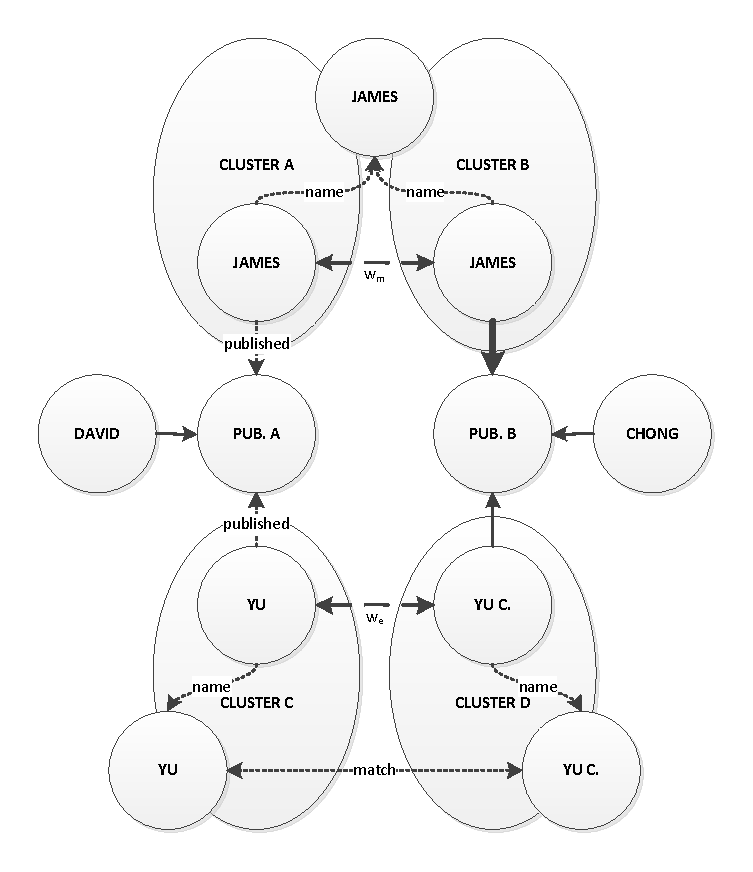
\includegraphics[width= 0.35\textwidth]{fig/coauthorrulenameeq.pdf}
	\caption{The co-author rule in action: comparing the two instance of James, a similarity ($w_m$) is added as the co-authors Yu and Yu C. match.}
	\label{fig:pipes}
\end{figure}

Rules are triggered by different events in the system. A rule could for example be executed when it has been discovered that an instance has published a publication, but could be executed on the event of a reclustering as well. The latter is a message that is a byproduct of the system itself and not originating from an external source.

Rules can be performed on three different scopes: instances with the same name, instances with similar names and instances part of the same cluster. That means that the instances of those collections are compared with the concerning instance. Strictly respecting this scopes narrow down the problem domain.

\section{Pipes and Filters}
\label{pipes}

The core of the implementation of the framework is the simplicity achieved by pipes and filters. They allow for modifiability and extensibility as pipes processing new sources or calculating new similarities between instances can easily be added to the system. An overview of the different pipes and the flow that runs between them is shown on \autoref{fig:pipes}. The expressiveness of StatefulPipe and the scalability of AsyncConnection in combination with a shared key-value store enables out-of-the-box and carefree scalability.

\begin{figure}[hb!]
	\centering
	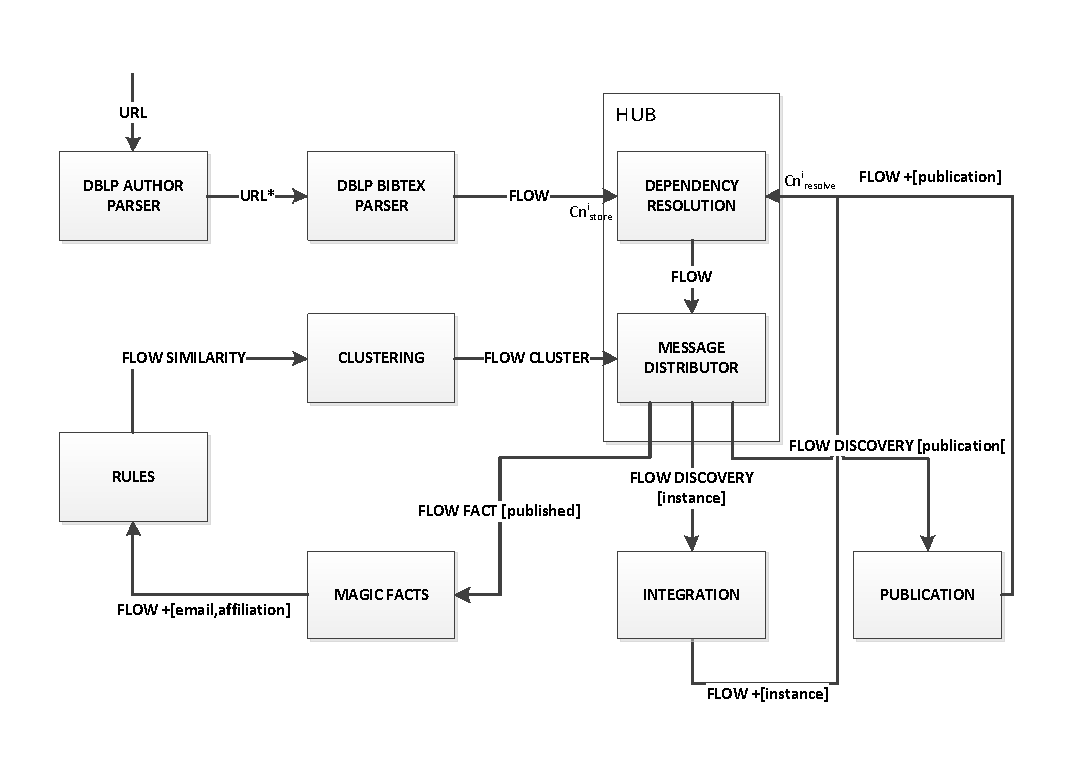
\includegraphics[width= 0.35\textwidth]{fig/completepipesmall.pdf}
	\caption{An overview of the different pipes and the flow running between them.}
	\label{fig:pipes}
\end{figure}

\section{Clustering}

The article focuses a lot on the clustering process. This process is responsible for calculating which instances match to the same author, based on similarities between the instances. Every time a rule computes a new similarity, it is possible reclustering has to occur. As there is a constant influx of information, there is a need for a dynamic approach that maintains the cluster quality. 

The article gives an in-depth explanation of the dynamic clustering algorithm described in \cite{dyncluster}. The algorithm itself depends on the minimum cut tree algorithm. The sequential Gusfield's algorithm described in \cite{gusfield} is implemented. 

The article also proposes an addition to the original clustering algorithm. It introduces a new case, acting the same as case 1, but being executed instead of case 3 on the occasion that $2 * \frac{cutvalue(C_v, C_u)}{\left|V\right|} <= \alpha / 2$. This anticipates the fact that a lot of similarities with lower weights occur and they often take place in succession. Often this results in case 3 being calculated multiple times in succession, before finally merging the clusters together. By introducing this new case, the resource-intensive execution of case 3 is swapped for the very fast execution of case 1.

The clustering process is implemented as a stateful pipe and is not treated any different from the other pipes. The clustering process is completely decoupled from the graph representation. Better yet, the graph is almost not being accessed during the clustering process. The reasoning about the grouping of instances is done completely local and the state of the similarities (the similarity plane) is maintained in the shared key-value store. This approach takes a lot of load off the database, which is important as a graph database does not scale that easily.

\section{Results}

\begin{figure}[htpb!]
\centering
%\includegraphics[width= 0.4\textwidth]{fig/performance_total.pdf}
\caption{Performance test of the matchmaker on Laptop (2GHz processor, 1GB RAM) and ALIX (500MHz processor, 256MB RAM)}
\label{fig:testperformance}
\end{figure}


\begin{figure}[htpb!]
\centering
%\includegraphics[width= 0.4\textwidth]{fig/parameters_en.pdf}
\caption{Test of influence of parameters on performance on Laptop (2GHz processor, 1GB RAM)}
\label{fig:testparameters}
\end{figure}



\section{Conclusions and future work}


%\nocite{*}
\bibliographystyle{phdsymp}
%%%%%\bibliography{bib-file}  % commented if *.bbl file included, as
%%%%%see below


%%%%%%%%%%%%%%%%% BIBLIOGRAPHY IN THE LaTeX file !!!!! %%%%%%%%%%%%%%%%%%%%%%%%
%% This is nothing else than the phdsymp_sample2e.bbl file that you would%%
%% obtain with BibTeX: you do not need to send around the *.bbl file        
%%
%%---------------------------------------------------------------------------%%
%
\begin{thebibliography}{1}
%\bibitem{paper}
%Bart Lannoo, Didier Colle, Mario Pickavet, Piet Demeester,
%\newblock {\em Optical Switching Architecture to Implement Moveable Cells in a Multimedia Train Environment},
%\newblock Proc. of ECOC 2004, 30th European Conf. on Optical Communication, vol. 3, pp. 344-345, Stockholm, Sweden, 5-9 Sep. 2004.
%
\bibitem{upnp}
Donoho A, Costa-requena J, Mcgee T, Messer A, Fiddian-green A, Fuller J. \newblock{\em UPnP Device Architecture 1.1.} Oct. 2008. 

\bibitem{cling}
Bauer C. \newblock{\em Cling UPnP.} 22 Mar. 2011. Available from: http://teleal.org/projects/cling/

\bibitem{owl}
Smith M, Welty C, McGuinness D. \newblock{\em OWL - Web Ontology Language.} 5 Apr. 2011. Available from: http://www.w3.org/TR/owl-guide/

\bibitem{owls}
Martin D, Burstein M, Hobbs J, Lassila O, McDermott D, McIlraith S, et al. \newblock{\em OWL-S - Semantic Markup for Web Services.} 21 Sep. 2010. Available from: http://www.w3.org/Submission/OWL-S/

\bibitem{owlstc}
SemWebCentral. \newblock{\em OWL-S Service Retrieval Test Collection: Project Info.} May 16 May. 2011. Available from: http://www.semwebcentral.org/projects/owls-tc/



%
%\bibitem{click}
%\newblock {\em The Click Modular Router Project},
%\newblock http://www.read.cs.ucla.edu/click/
%
%\bibitem{ns}
%\newblock {\em {NS} -- {N}etwork {S}imulator},
%\newblock http://nsnam.isi.edu/nsnam/
\end{thebibliography}
%
%%---------------------------------------------------------------------------%%

\end{document}

%%%%%%%%%%%%%%%%%%%%%  End of phdsymp_sample2e.tex  %%%%%%%%%%%%%%%%%%%%%%%%%%%

\bibliography{collection}
\backmatter
\end{document}
